\section{Implementácia}

Projekt ViDA vznikol ako ročníkový projekt a nevychádzal zo žiadnych predošlých prác alebo
projektov. Ako to vyzerá, môžete vidieť na obrázkoch.
Naším prvoradým cieľom, bolo zabezpečiť prehľadnú vizualizáciu a tiež jednoduché
používanie aplikácie.

\noindent
\begin{figure*}
\centering
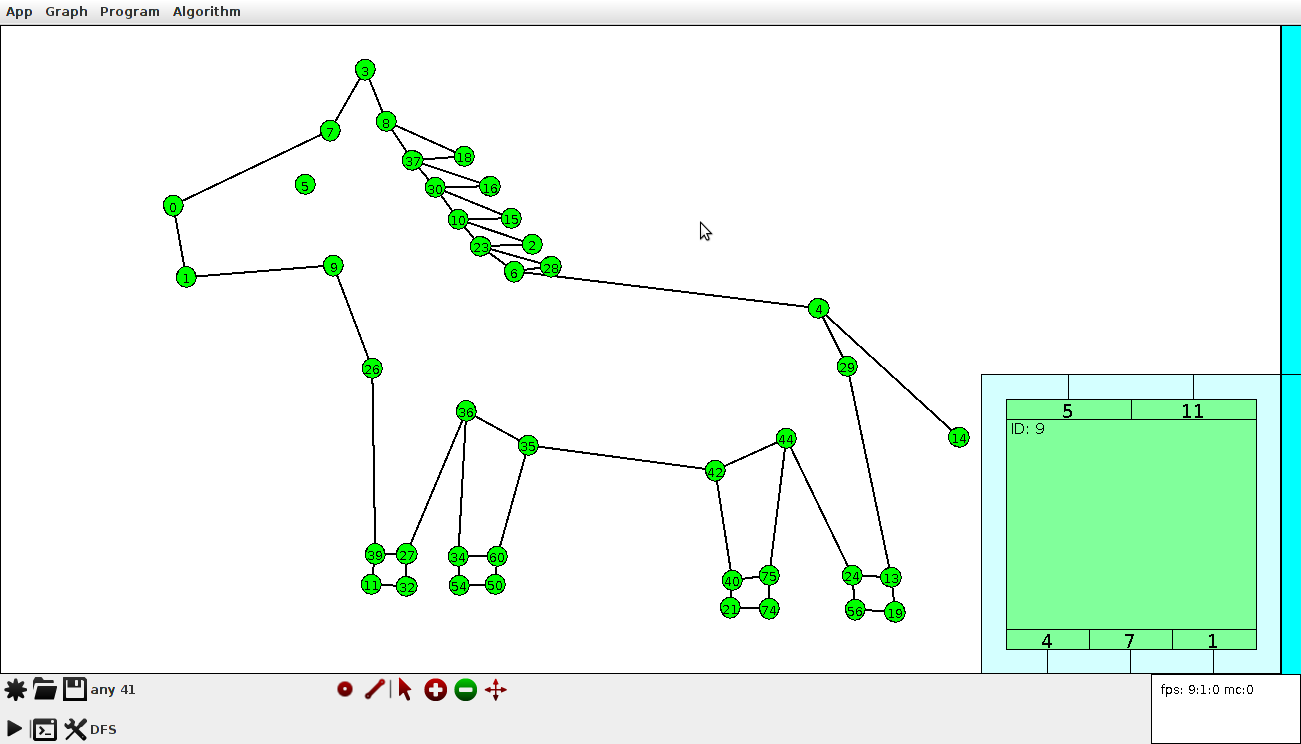
\includegraphics[width=2.01\columnwidth]{konik-je-uzasny.png}
\caption{\emph{Softvér ViDA.} Grafické rozhranie bez bežiacej vizualizácie, kde si užívateľ môže
nastaviť vzhľad svojho grafu -- napríklad aj na takéhoto pekného koníka. V ovládacej lište má
nástroje na vytváranie grafu a tiež nahrávanie programu, ktorý chce spúšťať. Napravo je informačné
okienko s dodatkovými informáciami o vrchole, teraz len s hodnotou id.}
\label{img:historia} 
\end{figure*}
%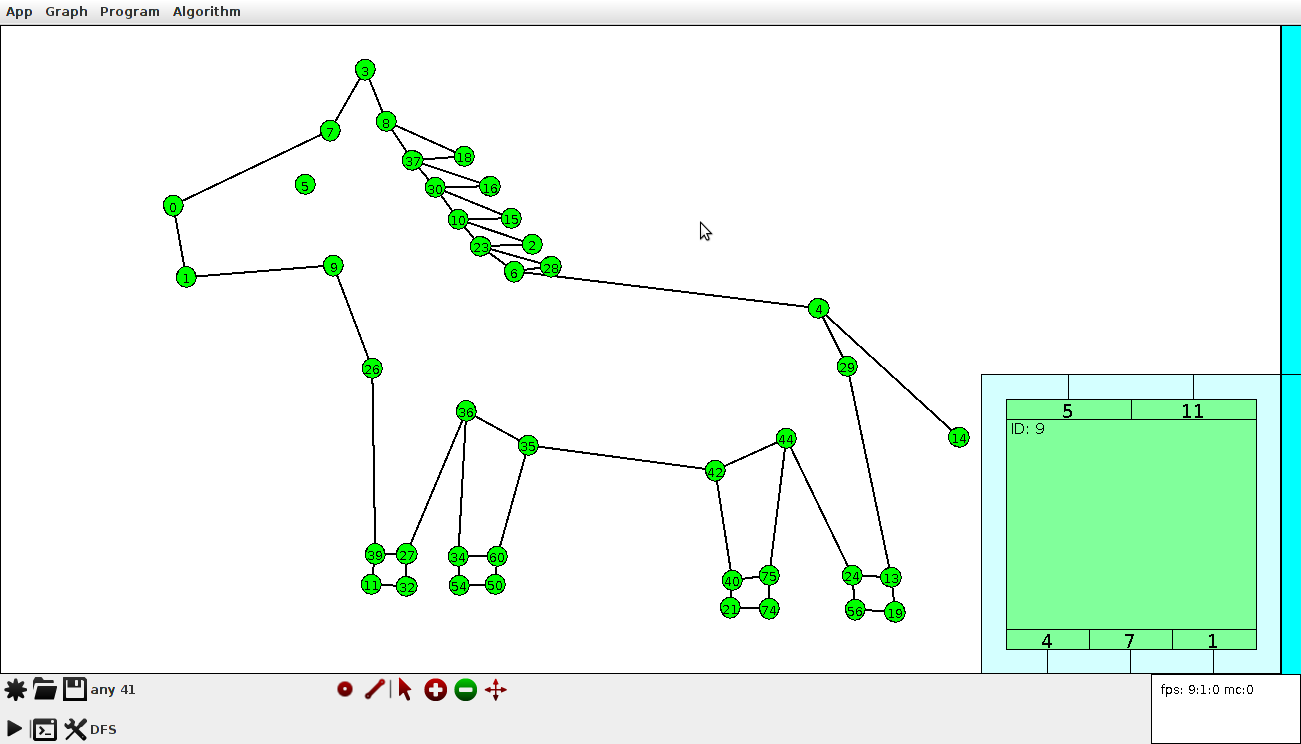
\includegraphics[width=8.5cm]{konik-je-uzasny.png}

\subsection{Vizualizácia}

Pri distribuovaných algoritmoch sa bavíme o sieti počítačov, ktoré medzi sebou komunikujú --
posielajú si medzi sebou správy. Preto bolo prirodzené, aby sme si reprezentovali počítače a ich
vzájomné zapojenie do siete ako graf. Každý vrchol je jeden počítač (proces) a správy sa presúvajú
medzi počítačmi, len po hranách v danom grafe.

Keďže samotná sieť počítačov má veľký vplyv na vykonávanie daného algoritmu, v prvej fáze, bolo
treba umožniť užívateľovi si pohodlným spôsobom vytvárať a editovať graf. Na to je určená hlavná
plocha, kde v dobe keď nebeží žiaden algoritmus, môže pomocou myši meniť výzor grafu. Na spodnej
lište je niekoľko tlačidiel, ktoré umožňujú užívateľovi prepínať si medzi možnosťami pridávanie,
odstraňovanie alebo pohybovanie. S vybratým módom, môže užívateľ vykonávať danú operáciu na grafe.
Takisto, existuje pár známych a často používaných typov grafov, ktoré si užívateľ môže zvoliť priamo
aj s danou veľkosťou grafu.

Samozrejme najdôležitejšia časť je vizualizácia samotného algoritmu. Bolo dôležité aby to bolo čo
najprehľadnejšie a zároveň to dávalo dostatok informácií. Z viacerých možností, ktoré sme skúšali
sme nakoniec vybrali bublinkový interface, kde všetky podstatné informácie sú zobrazované vo
vyskakovacích bublinkách.

Počas algoritmu jednotlivé procesy často oznamujú nejakú informáciu, aby dali najavo, čo sa v nich
deje. Zo začiatku sme tieto informácie zobrazovali v okienku napravo, aby sme nezahltili priestor
grafu zbytočnými textami. Toto všeobecné okienko bolo však mimo grafu a bolo skoro nemožné sledovať
čo sa deje vnútri grafu (kde ide aká správa) a zároveň si dávať pozor, čo vraví ktorý vrchol. Preto
sme sa rozhodli, že informácie vrchola sa budú zobrazovať priamo pri vrchole vnútri grafu, čo sa
nakoniec ukázalo, že až tak nezavadzá, hlavne ak tieto správy časom miznú. Ponechali sme aj
panel naboku, ktorý má slúžiť, keď si chce užívateľ pozrieť, čo sa dialo v histórii. A tento panel
nezavadzá, keďže je decentne skrytý a ukáže sa až na užívateľov príkaz.

Pri distribuovaných algoritmoch nás zaujíma hlavne to, ako sa algoritmus presúva z jedného stavu do
druhého na základe doručenej správy. Pod pojmom stav rozumiem naplnenie niektorých dôležitých
premenných. Je teda zjavné, že je dôležité, aby užívateľ videl (alebo aspoň tušil), akú hodnotu majú
tieto dôležité premenné. Dôležité premenné sú napríklad $id$ vrchola, či je živý alebo nie, jeho
level \dots Vypisovať tieto premenné v bublinkách pri vrchole, by však zavadzalo, keďže je to
informácia, ktorá je potrebná stále. Preto sme zvolili taký prístup, aby výzor vrcholu reprezentoval
dané premenné.

Keďže $id$ vrchola je jedna z najdôležitejších informácii, lebo je nezávislá od algoritmu, ktorý je
spustený a teda často slúži na prelomenie určitej symetrie, táto hodnota sa vypisuje priamo vnútri
vrchola. Ďalšie atribúty vrcholu sú jeho farba, alebo veľkosť. Preto naše vizualizácie často
využívajú tieto vlastnosti a intuitívne ich spájajú s nejakou premenou. Napríklad mŕtvy proces zmení
svoju farbu na červenú, alebo zväčšujúci sa level zväčšuje veľkosť vrchola.
Samozrejme, občas je dôležité aby sa užívateľ mohol pozrieť na skutočnú hodnotu danej premennej.
Preto si vie označiť vrchol, ktorý mu vo vedľajšom okienku ukáže premenné daného procesu.

Poslednou dôležitou vlastnosťou, ktorú bolo treba užívateľovi poskytnúť je možnosť časovať si
správy. Časovanie a poradie doručovania pošty do značnej formy ovplyvňuje priebeh a je dôležité aby
mal užívateľ možnosť ovplyvňovať toto dianie. Tak si vie sám vyrábať rôzne obskurné prípady,
poprípade svoj vlastný "worstcase".

Počas vývoja aplikácie aj táto funkcia prešla viacerými zmenami. Tak ako u všeobecných informácii
začínala oddelene od hlavného okna, v paneli kde sa zhromažďovali všetky správy. Avšak takisto sme sa
nakoniec rozhodli (vďaka Kuko), že bude lepšie to odtiaľ odstrániť, keďže sa to nedalo sledovať
simultánne. Preto sme to vložili priamo do plochy, takže stačí vybrať správu, chytiť ju myškou a
posunúť ju smerom, ktorým chceme. Samozrejme, že s ohľadom na výpočtový model kde pracujeme je
nemožné aby sa správy na jednej linke predbiehali.

\subsection{Knižnica vidalib}

Dôležitou súčasťou sú samozrejme jednotlivé algoritmy, ktoré chceme vizualizovať. Aj kvôli tomuto bolo
treba vymyslieť vhodný spôsob na písanie daných algoritmov. Jednou možnosťou ich bolo priamo zahrnúť
do aplikácie. Táto možnosť sa nám však videla príliš obmedzujúca pre užívateľa. Naším cieľom je aj
to, aby užívateľ mohol sám vytvoriť program, ktorý si vie spustiť a odvizualizovať vďaka našej
aplikácii. Za týmto účelom vznikla C++ knižnica \verb!vidalib.h!. Rozhodli sme sa, že zatiaľ sa samotné
algoritmy budú implementovať v C++, jednak kvôli rýchlosti a zároveň kvôli rozšírenosti a našej
osobnej obľuby. Vďaka návrhu aplikácie však nie je problém v budúcnosti pridať podporu pre viaceré
programovacie jazyky alebo ľubovoľné spustiteľné binárky.

V súčastnosti, keď chce užívateľ naprogramovať vlastný algoritmus, musí naimplementovať dve funckie: \verb!init()! a
\verb!recieve(port, message)!. Prvá sa zavolá na začiatku algoritmu a slúži na nastavenie
inicializačných premenných. V prípade broadcastu alebo traversalu sa program dozvie, či vlastní správu poprípade token.
Do tejto funkcie sa zvykne písať to, čo má program spraviť po naštartovaní.
Druhú volá naša knižnica vždy, keď príde nová správu, pričom ako parametre sa jej nastavia číslo
portu, po ktorej správa prišla a jej obsah. Proces môže posielať správy pomocou knižničnej
funkcie \verb!sendMessage(port, message)!.

Toto je už postačujúce k tomu, aby užívateľ mohol napísať program, ktorý by vedel spustiť našou
aplikáciou a ktorý by fungoval. Nebol by však schopný ovplyvňovať vizualizáciu. Aby sme mu umožnili
aj toto, pridali sme do našej knižnice ďalšie funkcie. Konkrétne vie užívateľ meniť veľkosť a farbu
vrcholu grafu, prinútiť pozastaviť vykonávanie programu, aby upozornil na dôležitú udalosť a
taktiež posielať texty, ktoré sa majú vypisovať pri vrchole.

Takisto sme zaviedli takzvané \verb!WatchVariables!. Sú to premenné, ktoré si užívateľ určí, že sú
dôležité a chce, aby sa zobrazovali pri podrobnostiach vrcholu. K týmto premenným má
prístup, cez našu knižnicu. Výnimkou je $id$ vrchola, ktoré je dané explicitne, nemožno ho
meniť a je zobrazované vždy. Samozrejme užívateľ môže používať ľubovoľné ďalšie premenné.

Týmto dávame užívateľovi skoro taký istý arzenál na vizualizáciu, aký používame my. Dávame mu teda
možnosť tešiť sa z úspešného programu, ktorý sa pekne vizualizuje rovnako, ako sme sa tešili my, keď
nám začali behať naše prvé algoritmy. A o tom, čo máme oproti užívateľovi naviac si povieme v
nasledujúcej podsekcii.

\subsection{Popis algoritmov}

Na jednej strane je dôležitá samotná vizualizácia -- jej prehľadnosť a názornosť. Na druhej strane
je však potrebné všetko vysvetliť aj pomocou popisu. Toto je zároveň jediná vec, ktorú užívateľ
zatiaľ nevie robiť a je dostupná len pre nami robené programy. Uvažujeme však aj o tom, že v budúcnosti
ju tiež umožníme ovplyvňovať užívateľom.

Dôležité bolo zamyslieť sa nad tým, ako čo najnázornejšie popísať, čo sa práve v algoritme deje.
V tejto fáze sme si predstavovali, ako by sme dané algoritmy vysvetľovali niekomu inému, dokonca sme si to priamo
vyskúšali na sústredení KSP. Zhodnotili sme, že vysvetľovanie prebieha náčrtom hlavnej myšlienky,
teda čo je cieľ, ktorý sa každý program snaží dosiahnuť. Následne sme vysvetľovali jednotlivé prípady, ktoré
môžu nastať a ako sa riešia.

Rozhodli sme sa použiť túto ideu a pre každý algoritmus sme si vytvorili množinu rôznych prípadov,
ktoré môžu nastať. Náš program v C++ posiela informácie o tom, či nastala niektorá z týchto udalostí
a aplikácia na ňu patrične reaguje. Väčšinou, ak sa tento prípad vyskytol prvýkrát, program sa
zastaví a v bublinke sa vypíše text, ktorý upozorňuje na danú udalosť a tiež hovorí, čo sa bude
diať ďalej. Toto umožňuje užívateľovi sa pripraviť na to, čo sa bude diať a následne sa vie pozrieť
či sa to skutočne stalo a aké to malo dôsledky. Takto si užívateľ môže prezrieť všetky zaujímavé
prípady, ktoré môžu nastať a pochopiť aj zvyšné detaily algoritmu.

Dokonca užívateľ vie jednoducho ovplyvňovať to, ktoré prípady nastanú, nastavovaním rýchlostí
jednotlivých správ.

Taktiež sme rozmýšľali, či vieme nejak znázorniť, že algoritmus naozaj pošle očakávaný počet správ.
Jedna vec je totiž povedať, že to bude $O(n\log n)$, na druhej strane máme však reálny počet správ,
ktoré sa pošlú. A keď pošle algoritmus $100$ správ nedá sa veľmi dobre ukázať, že to patrí do $O(n
\log n)$ a nie do $O(n)$ s vysokou konštantou.

Tento konkrétny problém sme riešili hlavne v algoritme na hľadanie šéfa v úplnom grafe. Namiesto
zložitého rozpisovania dôkazu sme zobrali jeho hlavnú myšlienku a pokúsili sa ju názorne ukázať.
Hlavná myšlienka spočíva v tom, že vrcholov na nejakom leveli je najviac niekoľko. Preto počas behu
algoritmu počítame počet vrcholov na danom leveli. Následne ukážeme, že ich je menej ako očakávaný
počet z čoho vyplýva daná zložitosť. Samozrejme nie je to exaktný dôkaz, ale dáva to užívateľovi
hlbšie pochopenie na príkladoch. Môže sa napríklad snažiť, pomocou časovania správ vytvoriť čo
najhorší prípad, aby sa
presvedčil, že aj na ňom to funguje.

\noindent
\begin{figure*}
\centering
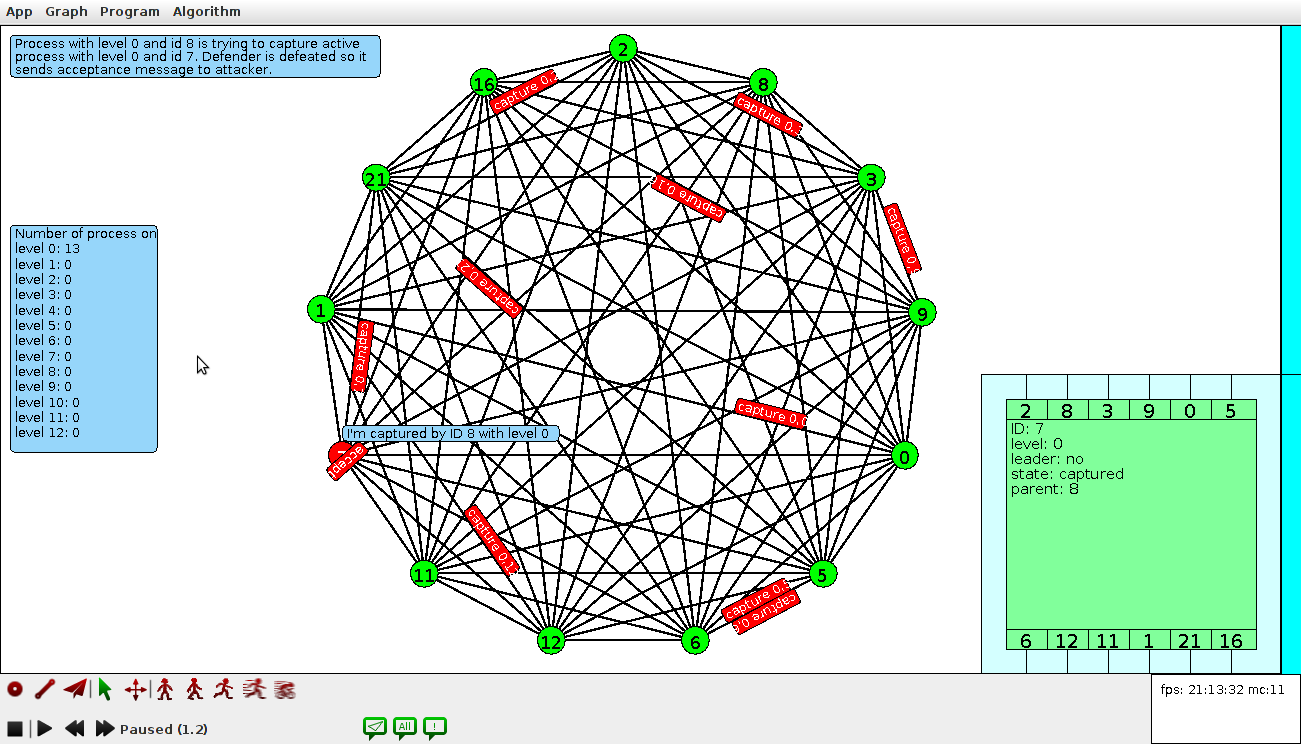
\includegraphics[width=2.01\columnwidth]{LE.png}
\caption{\emph{Softvér ViDA.} Algoritmus na voľbu šéfa. Bol pozastavený, aby užívateľovi
vysvetlil, čo sa práve deje v informačnej bublinke v ľavom hornom rohu. Naviac si vľavo počíta koľko
vrcholov bolo na danom leveli, aby znázornil efektívnosť algoritmu.}
\label{img:historia} 
\end{figure*}
%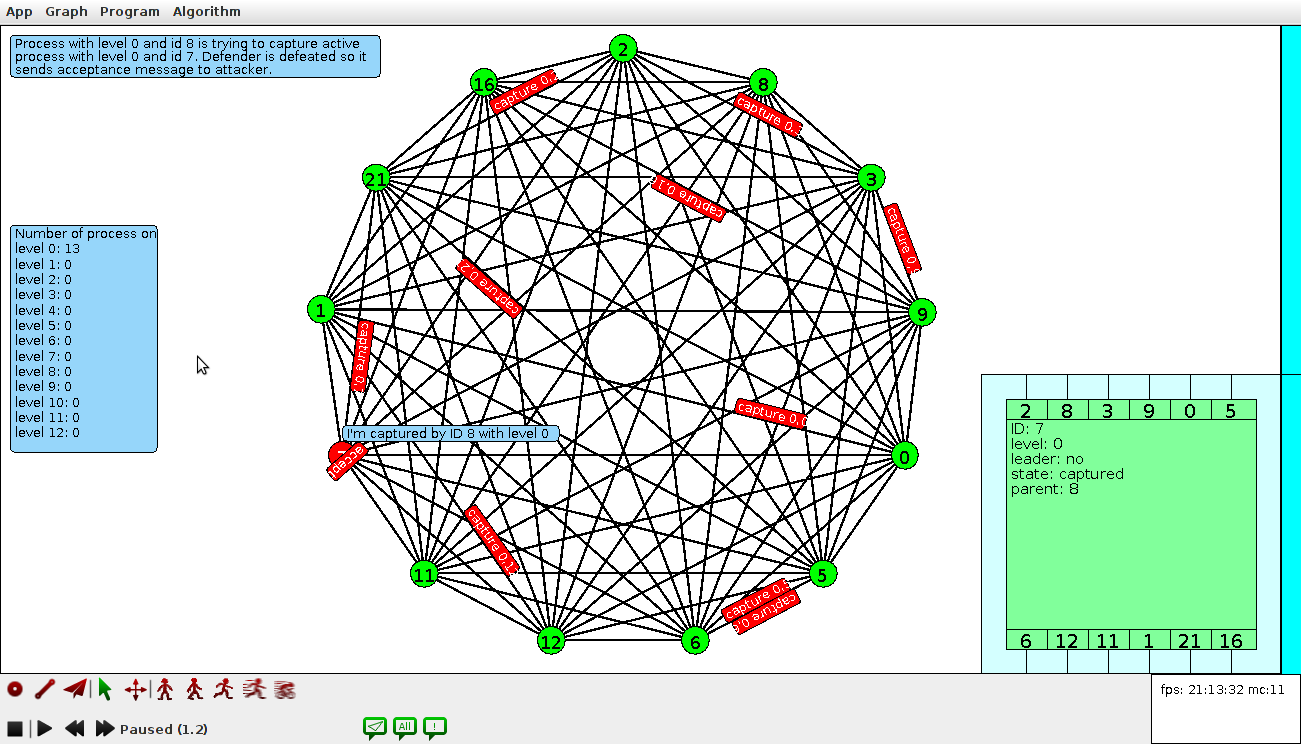
\includegraphics[width=8.5cm]{LE.png}
